\chapter{Visualizing 2D interpolation}

% Authors: Pedro Manuel Herrero Vidal, Doruk Kilitcioglu
% Lecture date: 2/27/2019

We take the data simulated in the 04-spiral\_classification notebook (\href{https://github.com/Atcold/pytorch-Deep-Learning-Minicourse/blob/master/04-spiral\_classification.ipynb} {"Spiral Classification"}), 
consisting of 3,000 samples of dimension 2 (Fig. ~\ref{fig:NonLinearlySeparableParametricCurves2}). 
The data is generated from the following expression:

\[
X_c(t) = t
\begin{bmatrix}
    \sin{\frac{2\pi}{C} (2t+c+1) + \mathcal{N} (0, \sigma^2)} \\
    \cos{\frac{2\pi}{C} (2t+c+1) + \mathcal{N} (0, \sigma^2)}
\end{bmatrix}
\]
%\noindent
where $0 \leq t \leq 1$ and classes $c=1, ..., C$.


\begin{figure}[ht]
\centering
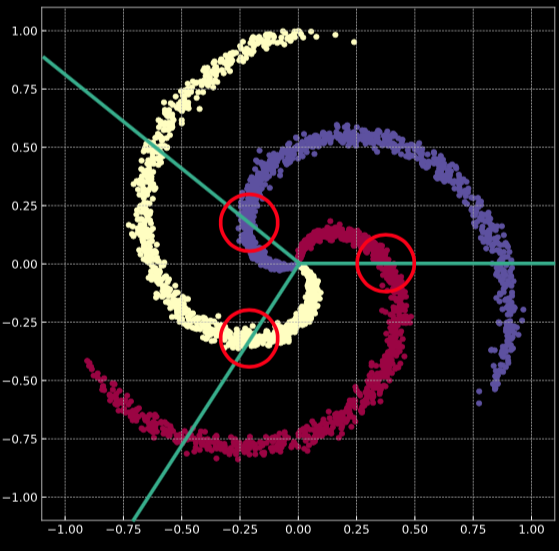
\includegraphics[width=0.5\textwidth]{figs/NonLinearlySeparableParametricCurves.png}
\caption{3 non linearly separable curves consisting in 3,000 samples from $X \in {{\rm I\!R}}^2$.}
\label{fig:NonLinearlySeparableParametricCurves2}
\end{figure}

\noindent
To classify the data into the three categories, we are going to use a three layer net with: 
\begin{itemize}
\item[(1)] 2 input units (dimensionality of the data).
\item[(2)] A 100-units hidden layer (used to increase the space and extract features).
\item[(3)] Followed by a non-linear ReLU activation function. 
\item[(4)] We then go back down to 2D again which is useful for visualization.
\item[(5)] Lastly we can bring it back up to 3D with a final linear transformation to a 3-unit output layer with softmax activation function for classification 
(Fig. ~\ref{fig:ArchitectureForClassificationAndVisualizationInTheInputSpace}). 
The last linear transformation involves the multiplication of $\matr{A^{(2)}}$ and $\matr{W^{(2)}}$, 
where the different rows of $\matr{W^{(2)}}$ are the 2D vectors that will point at the different classes in the 2D space. 
In this representation, the different classes are linearly separable.
\end{itemize}

\begin{figure}[!h]
\centering
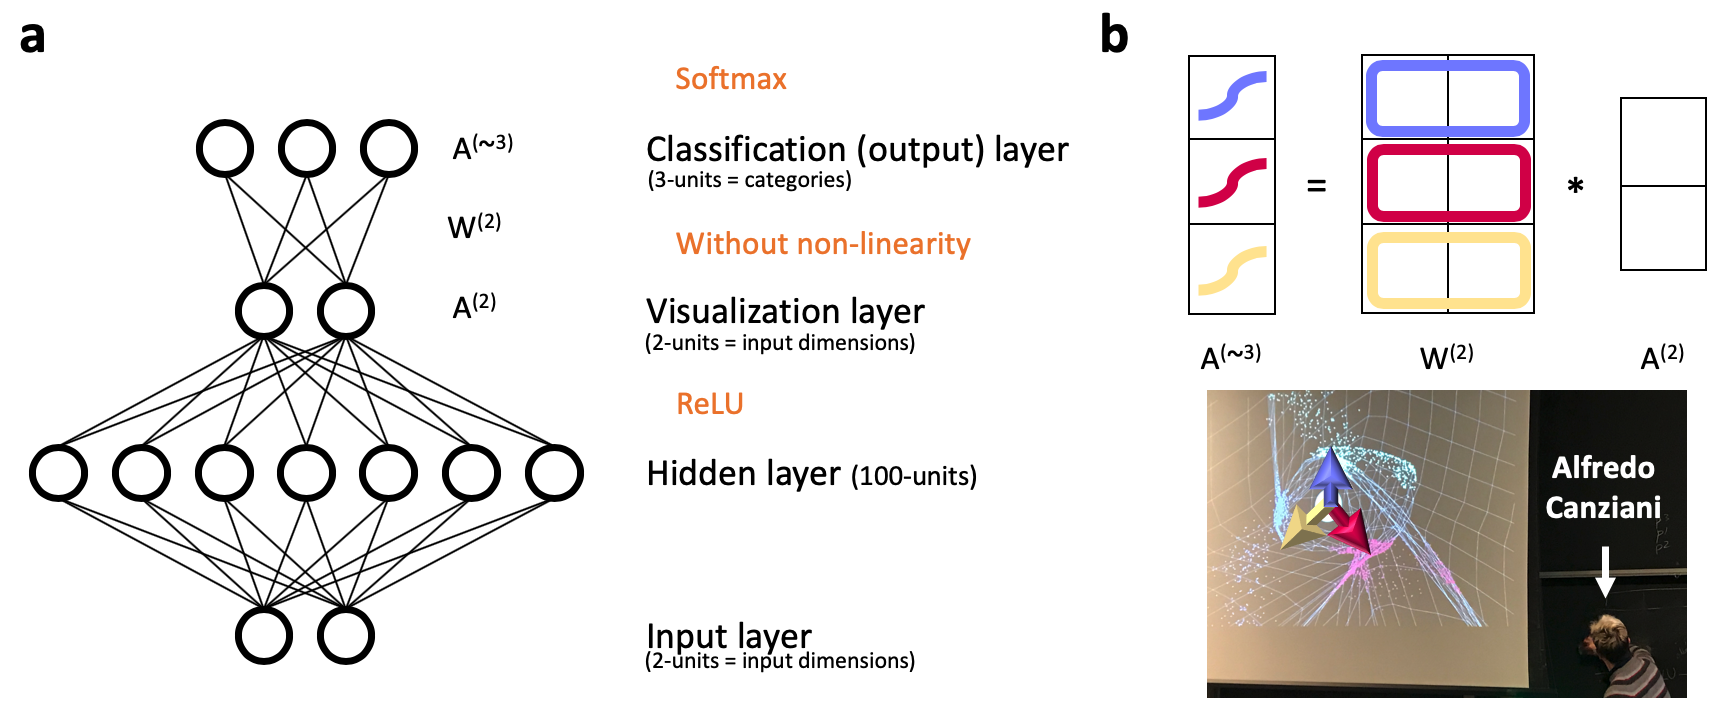
\includegraphics[width=170mm]{figs/ArchitectureForClassificationAndVisualizationInTheInputSpace.png}
\caption{Neural network architecture for classification and visualization in the input space. (a) Architecture of the neural network, which takes 2D inputs and visualizes in the same dimensional space before classification. (b) Linear transformation that takes $\matr{A^{(2)}}$ and returns $\matr{A^{(3)}}$ via multiplication with $\matr{W^{(2)}}$. Rectangular color boxes in $\matr{W^{(2)}}$ represent the three 2D vectors that will define each class. Calculation of $\matr{A^{(3)}}$ is followed by a softmax activation function for classification. In the bottom half of (b), the transformed data after and the population vectors (plot credit: Alfredo Canziani).}
\label{fig:ArchitectureForClassificationAndVisualizationInTheInputSpace}
\end{figure}

\noindent

In order to visualize each transformation, we do a linear interpolation from the input to the output at the 2D hidden layer using:

\[
(1-\alpha)(x^{(1)}) + \alpha \phi (x^{(i)}) ~~\text{ where } 0 \leq \alpha \leq 1
\]
